Die Zeitgleichung ist die Zeit, um die eine Sonnenuhr gegenüber einer
gleichmässig gehenden Uhr falsch geht.
Sie rührt daher, dass sich die Erde auf ihrer elliptischen Bahn um die
Erde nicht immer gleich schnell bewegt und kann mit Hilfe der keplerschen
Gesetze erklärt und berechnet werden.

Empirisch wurden für $N=12=2\cdot 6$ über das Jahr gleichmässig verteilte
Tage folgende Werte für die Zeitgleichung gefunden:
\begin{center}
\begin{tabular}{|c|>{$}r<{$}||c|>{$}r<{$}|}
\hline
Datum&\Delta t\;[\text{min}]&Datum&\Delta t\;[\text{min}]\\
\hline
1.~1.& -3.2&4.~7. &-4.1\\
1.~2.&-13.6&3.~8. &-6.1\\
2.~3.&-12.3&3.~9. & 0.5\\
2.~4.& -3.9&3.~10.&10.7\\
3.~5.&  3.1&2.~11.&16.3\\
3.~6.&  2.0&2.~12.&10.6\\
\hline
\end{tabular}
\end{center}
Es sind bereits die folgenden Fourier-Koeffizienten berechnet worden:
\begin{center}
\begin{tabular}{|>{$}c<{$}|>{$}r<{$}|>{$}r<{$}|}
\hline
k&\hat a_k&\hat b_k\\
\hline
0& 0.000&\text{---}\\
1& 0.342&-7.528\\
2&-3.575&\phantom{-9.165}\\
3& 0.083&-0.250\\
4&-0.125&-0.159\\
5& 0.025&-0.022\\
6&\phantom{ 0.050}&\text{---}\\
\hline
\end{tabular}
\end{center}
\begin{teilaufgaben}
\item Berechnen Sie die fehlenden Koeffizienten $\hat a_6$ und $\hat b_2$.
\item Welche Frequenz (welches $k$) ist dominant?
\item Wie gross ist der Fehler, wenn man nur die Terme bis $k=2$
berücksichtigt?
\end{teilaufgaben}

\begin{loesung}
\begin{figure}
\centering
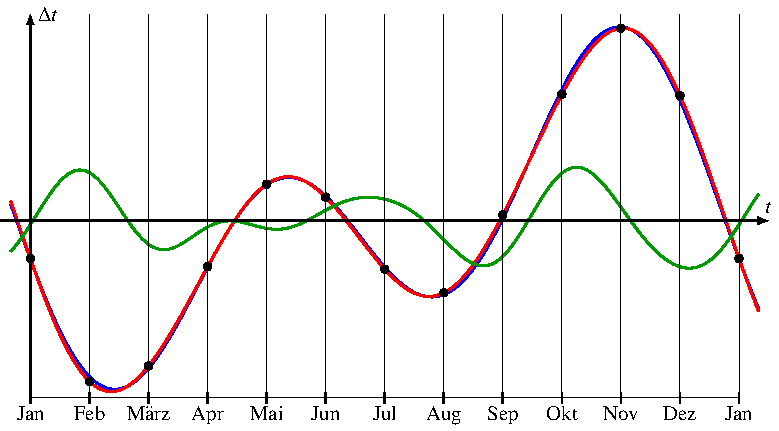
\includegraphics{chapters/060-diskret/images/zeitgl.pdf}
\caption{Zeitgleichung an über das Jahr gleichmässig verteilten Tagen
(schwarze Punkte).
Die rote Kurve zeigt eine Rekonstruktion mit Hilfe der diskreten
Fourier-Transformation.
Sie unterscheidet sich nur geringfügig von einem trignometrischen Polynom,
bei dem man nur die Terme bis $k=2$ berücksichtigt (blaue Kurve).
Der durch diese Näherung verursachte Fehler ist zehnfach überhöht in der
grünen Kurve dargestellt.
\label{zeitgleichung}
}
\end{figure}
\begin{table}
\centering
\begin{tabular}{|>{$}c<{$}|>{$}r<{$}| >{$}r<{$}| >{$}r<{$}|}
\hline
j &  y_j& \cos 6t_j&\sin 2t_j\\
\hline
0 & -3.2&         1& 0.00000\\
1 &-13.6&        -1& 0.86603\\
2 &-12.3&         1& 0.86603\\
3 & -3.9&        -1& 0.00000\\
4 &  3.1&         1&-0.86603\\
5 &  2.0&        -1&-0.86603\\
6 & -4.1&         1& 0.00000\\
7 & -6.1&        -1& 0.86603\\
8 &  0.5&         1& 0.86603\\
9 & 10.7&        -1& 0.00000\\
10& 16.3&         1&-0.86603\\
11& 10.6&        -1&-0.86603\\
\hline
  &     &\hat a_6=0.10&\hat b_2=-9.165\\
\hline
\end{tabular}
\caption{Tabelle zur Berechnung der Koeffizienten $\hat a_2$ und $\hat b_6$.
\label{koeftab}}
\end{table}
\begin{teilaufgaben}
\item
Es sind die Koeffizienten $\hat a_6$ und $\hat b_2$ zu berechnen.
Wir stellen die nötigen Daten in der Tabelle~\ref{koeftab} zusammen.
Dabei ist zu beachten, dass für $k=2$ die Winkel $t_j$ Vielfache von $60^\circ$
sind, deren Sinuswerte immer $\pm\!\sqrt{3}/2$ sind, man muss also nur 
die $y_j$ mit $j\in\{1,2,4,5,7,8,10,11\}$ mit den richtigen Vorzeichen
addieren und mit $\!\sqrt{3}/2$ multiplizieren.
Die Werte für $\hat a_6$ und $\hat b_2$ bekommt man aus
\begin{align*}
\hat a_6
&=
\frac{1}{12}
\sum_{j=0}^{11}
y_j (-1)^j
=
0.05
\\
\hat b_2
&=
\frac{2}{12}
\sum_{j=0}^{11}
y_j \sin 2\frac{2\pi j}{12}
=
-9.165
\end{align*}
\item
Die dominanten Terme sind $k=1$ und $k=2$.
Dies kann man auch in der Abbildung~\ref{zeitgleichung} erkennen, wo
ausser der Rekonstruktion mit allen Koeffizienten auch das
trigonometrische Polynom gezeigt ist, bei dem die Terme mit $k>2$ weggelassen
wurden.
Die Übereinstimmung ist immer noch sehr gut.
\item
Der Approximationsfehler ist bestimmt durch die die Terme 
\begin{align*}
|\vec{e}(t)|^2
&=
\sum_{k=3}^6 \hat a_k^2 \vec{c}_k\cdot\vec{c}_k
+
\sum_{k=3}^5 \hat b_k^2 \vec{s}_k\cdot\vec{s}_k
\\
&=
0.083^2\cdot 6
+0.125^2\cdot 6
+0.025^2\cdot 6
+0.05^2\cdot 12
+0.25^2\cdot 6
+0.159^2\cdot 6
+0.022^2\cdot 6
\\
&=
6\cdot 0.1164
=
0.6984
\\
|e(t)|
&=
0.83570
\end{align*}
Der mittlere Fehler der Approximation beträgt also weniger als eine Minute.
\qedhere
\end{teilaufgaben}
\end{loesung}

